% Part-Set Fusion V7 — working-principle / flow diagram (research-paper style)
% Build:  pdflatex v7_flow_diagram.tex
% All numbers (dimensions, parameter counts, metrics) are the real values from
% designs/skeleton_silhouette_partset_v7 and runs/.../partset_rank1_001.
\documentclass[tikz, border=10pt]{standalone}
\usepackage[T1]{fontenc}
\renewcommand{\familydefault}{\sfdefault}
\usetikzlibrary{positioning, calc, fit, backgrounds, decorations.pathreplacing, arrows.meta}

% ---- palette (paper-pastel) ----
\definecolor{encblue}{RGB}{174,199,232}
\definecolor{encblueD}{RGB}{68,114,196}
\definecolor{fusorange}{RGB}{255,214,130}
\definecolor{fusorangeD}{RGB}{191,128,22}
\definecolor{partgreen}{RGB}{178,219,180}
\definecolor{partgreenD}{RGB}{56,118,79}
\definecolor{temppurple}{RGB}{206,190,231}
\definecolor{temppurpleD}{RGB}{112,84,163}
\definecolor{headgray}{RGB}{233,233,233}
\definecolor{headgrayD}{RGB}{110,110,110}
\definecolor{lossred}{RGB}{192,28,28}
\definecolor{inkdark}{RGB}{45,45,45}

\tikzset{
  blk/.style={draw=#1!70!black, fill=#1, rounded corners=2.5pt, align=center,
              font=\scriptsize, inner sep=4pt, minimum height=9mm, line width=0.5pt},
  lbl/.style={font=\scriptsize\bfseries, text=inkdark, align=center},
  sub/.style={font=\tiny, text=inkdark!75, align=center},
  flow/.style={-{Stealth[length=2.2mm]}, line width=0.7pt, draw=inkdark},
  trainflow/.style={-{Stealth[length=2mm]}, line width=0.6pt, draw=headgrayD, dashed},
  lossdot/.style={circle, fill=lossred, inner sep=0pt, minimum size=1.7mm},
  losslbl/.style={font=\tiny, text=lossred, align=center},
  frame/.style={draw=inkdark!60, line width=0.4pt, inner sep=0pt},
}

\begin{document}
\begin{tikzpicture}[x=1cm, y=1cm]

% =========================================================== inputs
% silhouette stack
\node[frame] (silc) at (0.30, 6.70) {
\includegraphics[width=11mm]{assets/sil_c.png}};
\node[frame] (silb) at (0.15, 6.85) {
\includegraphics[width=11mm]{assets/sil_b.png}};
\node[frame] (sila) at (0.00, 7.00) {
\includegraphics[width=11mm]{assets/sil_a.png}};
\node[lbl, below=8.5mm of sila, xshift=1.5mm] (sillab) {silhouette sequence};
\node[sub, below=0.5mm of sillab] {$B \times 30 \times 1 \times 64 \times 64$};

% skeleton / topology stack
\node[frame] (skc) at (0.30, 2.30) {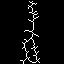
\includegraphics[width=11mm]{assets/skel_c.png}};
\node[frame] (skb) at (0.15, 2.45) {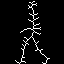
\includegraphics[width=11mm]{assets/skel_b.png}};
\node[frame] (ska) at (0.00, 2.60) {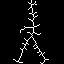
\includegraphics[width=11mm]{assets/skel_a.png}};
\node[lbl, below=8.5mm of ska, xshift=1.5mm] (skelab) {topology sequence};
\node[sub, below=0.5mm of skelab] {$B \times 30 \times 3 \times 64 \times 64$\\HJ skeleton $\cdot$ structure blur $\cdot$ motion};

% =========================================================== stems
\node[blk=encblue] (silstem) at (3.4, 6.85) {\textbf{Silhouette stem}\\Conv $1{\to}32{\to}64$, s2\\$64\,$ch @ $32{\times}32$};
\node[blk=encblue] (skstem)  at (3.4, 2.45) {\textbf{Skeleton stem}\\Conv $3{\to}32{\to}64$, s2\\$64\,$ch @ $32{\times}32$};

\draw[flow] (silc.east) -- (silstem.west);
\draw[flow] (skc.east)  -- (skstem.west);

% =========================================================== spatial gated fusion
\node[blk=fusorange, minimum height=16mm] (gate) at (6.6, 4.65)
  {\textbf{Spatial gated fusion}\\[1pt]
   $g=\sigma(\mathrm{Conv}_{1\times1}[\,\mathrm{sil},\mathrm{skel}\,])$\\
   $g \odot \mathrm{skel} + (1{-}g)\odot \mathrm{sil}$\\[1pt]
   per-pixel, per-channel};

\draw[flow] (silstem.east) -| ($(gate.north)+(0,0.0)$);
\draw[flow] (skstem.east)  -| (gate.south);

% =========================================================== shared trunk (bars)
\begin{scope}[shift={(8.7, 4.65)}]
  \draw[fill=encblue, draw=encblueD, rounded corners=1pt] (0.00,-1.30) rectangle (0.34, 1.30);
  \draw[fill=encblue, draw=encblueD, rounded corners=1pt] (0.55,-1.05) rectangle (0.89, 1.05);
  \draw[fill=encblue, draw=encblueD, rounded corners=1pt] (1.10,-1.05) rectangle (1.44, 1.05);
  \draw[fill=encblue, draw=encblueD, rounded corners=1pt] (1.65,-1.05) rectangle (1.99, 1.05);
  \node[sub] at (0.17, 1.55) {96};
  \node[sub] at (0.72, 1.30) {128};
  \node[sub] at (1.27, 1.30) {160};
  \node[sub] at (1.82, 1.30) {192};
  \node[sub] at (0.17,-1.55) {$32^2$};
  \node[sub] at (1.27,-1.30) {$16^2$};
  \node[lbl] at (1.0,-2.10) {shared trunk};
  \node[sub] at (1.0,-2.50) {fused map $192\,$ch @ $16{\times}16$};
  \coordinate (trunkin)  at (-0.15, 0);
  \coordinate (trunkout) at (2.14, 0);
\end{scope}
\draw[flow] (gate.east) -- (trunkin);

% =========================================================== part-set branch (top)
\node[blk=partgreen] (strips) at (12.6, 7.30)
  {\textbf{8 horizontal part strips}\\avg $+$ max pool per strip\\$B \times 30 \times 8 \times 192$};
\node[blk=partgreen] (setmax) at (16.1, 8.15)
  {\textbf{set-max over $T$}\\most discriminative\\appearance per part};
\node[blk=partgreen] (tconv) at (16.1, 6.35)
  {\textbf{temporal conv $\times 2$}\\(grouped, dilated) $+$ max\\short-range part motion};
\node[circle, draw=partgreenD, fill=white, inner sep=1pt, font=\scriptsize] (psum) at (18.35, 7.30) {$+$};
\node[blk=partgreen] (partfc) at (20.3, 7.30)
  {\textbf{per-part FC}\\$8 \times (192 {\to} 64)$\\$\Rightarrow$ 512-D};

\draw[flow] (trunkout) |- (strips.west);
\draw[flow] (strips.east) -| ($(setmax.west)+(-0.35,0)$) |- (setmax.west);
\draw[flow] (strips.east) -| ($(tconv.west)+(-0.35,0)$) |- (tconv.west);
\draw[flow] (setmax.east) -| (psum.north);
\draw[flow] (tconv.east)  -| (psum.south);
\draw[flow] (psum.east) -- (partfc.west);

% =========================================================== global temporal branch (bottom)
\node[blk=temppurple] (gap) at (12.6, 2.00)
  {\textbf{GAP per frame}\\$B \times 30 \times 192$};
\node[blk=temppurple] (tcnn) at (15.35, 2.00)
  {\textbf{temporal Conv1d}\\grouped, $k{=}3$};
\node[blk=temppurple] (gru) at (18.15, 2.00)
  {\textbf{Bi-GRU}\\2 layers, $h{=}176$\\$B \times 30 \times 352$};
\node[blk=temppurple] (pool) at (20.95, 2.00)
  {\textbf{attn $+$ mean pool}\\$\Rightarrow$ 704-D};

\draw[flow] (trunkout) |- (gap.west);
\draw[flow] (gap.east) -- (tcnn.west);
\draw[flow] (tcnn.east) -- (gru.west);
\draw[flow] (gru.east) -- (pool.west);

% =========================================================== concat + embedding
\node[circle, draw=inkdark, fill=white, inner sep=1.5pt, font=\scriptsize\bfseries] (cat) at (22.6, 4.65) {$\oplus$};
\node[blk=headgray, minimum height=13mm] (emb) at (24.5, 4.65)
  {\textbf{embedding MLP}\\$1216 {\to} 512 {\to} 256$\\LN $\cdot$ GELU $\cdot$ BN};
\node[draw=inkdark, fill=white, rounded corners=2.5pt, align=center, inner sep=4pt,
      font=\scriptsize\bfseries, line width=0.8pt] (embvec) at (27.55, 4.65) {256-D gait\\embedding};

\draw[flow] (partfc.east) -| (cat.north);
\draw[flow] (pool.east)   -| (cat.south);
\draw[flow] (cat.east) -- (emb.west);
\draw[flow] (emb.east) -- (embvec.west);

% =========================================================== training heads
\node[blk=headgray] (proj) at (27.55, 7.05)
  {\textbf{projection head}\\$256 {\to} 128$, $\ell_2$-norm};
\node[blk=headgray] (clf) at (27.55, 2.35)
  {\textbf{classifier} (train only)\\$256 {\to}$ \#subjects};
\node[blk=headgray, minimum height=12mm] (dec) at (21.3, 0.20)
  {\textbf{skeleton decoder} (train only)\\ConvT $\times 3$: reconstructs masked\\skeleton $+$ motion frames};

\draw[flow] (embvec.north) -- (proj.south);
\draw[flow] (embvec.south) -- (clf.north);
\draw[trainflow] (gru.south) |- ($(dec.west)+(-0.3,0)$) -- (dec.west);
\node[sub, text=headgrayD] at (16.3, 0.30) {30\,\% of frames masked\\on generative steps};

% loss dots
\node[lossdot] (l1) at ($(proj.north)+(0,0.35)$) {};
\node[losslbl, right=1.2mm of l1] {$\mathcal{L}_{\mathrm{SupCon}}$};
\node[lossdot] (l2) at ($(embvec.east)+(0.55,0.80)$) {};
\node[losslbl, above=0.8mm of l2] {$\mathcal{L}_{\mathrm{triplet}}$\\(batch-hard)};
\node[lossdot] (l3) at ($(clf.south)+(0,-0.35)$) {};
\node[losslbl, right=1.2mm of l3] {$\mathcal{L}_{\mathrm{CE}}\ (\lambda{=}0.12)$};
\node[lossdot] (l4) at ($(dec.east)+(0.40,0)$) {};
\node[losslbl, right=1.2mm of l4] {$\mathcal{L}_{\mathrm{recon}}$: wBCE $+$ Dice $+$ SmoothL1};

% =========================================================== retrieval output
\node[frame] (pca) at (31.6, 4.65) {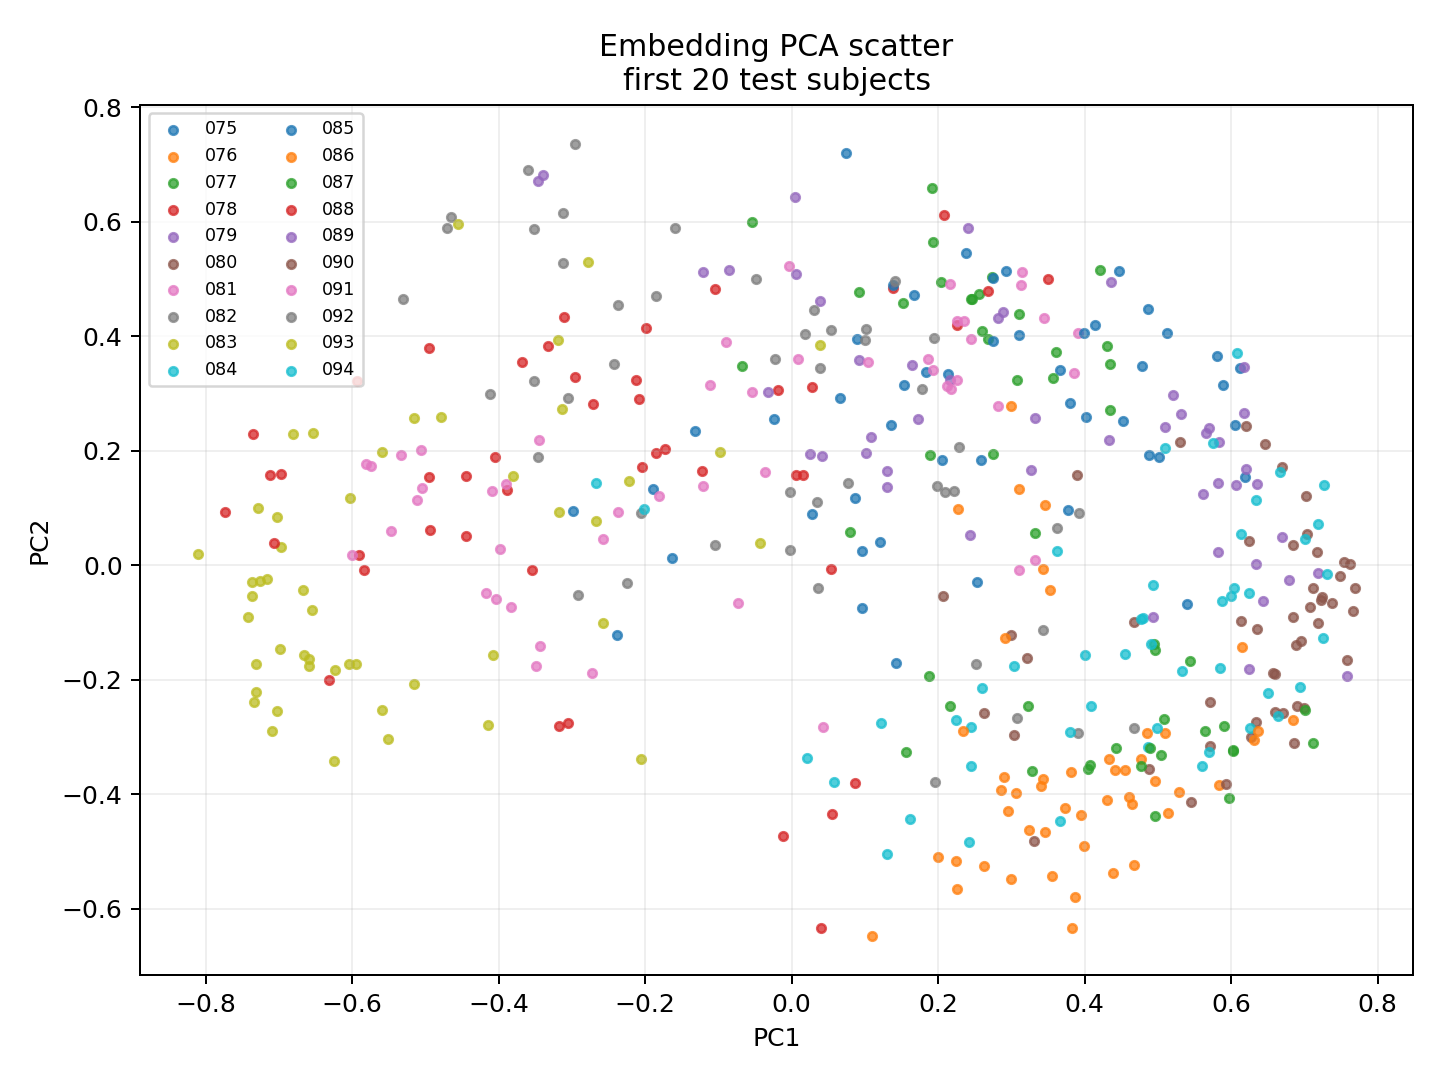
\includegraphics[width=28mm]{assets/pca.png}};
\node[lbl, below=1mm of pca] (pcalab) {cosine-distance retrieval};
\node[sub, below=0.2mm of pcalab] {same person close $\cdot$ different person far\\Rank-1 / Rank-5 / verification AUC};
\draw[flow] (embvec.east) -- node[sub, above, yshift=0.5mm] {eval} (pca.west);

% =========================================================== info box (top right)
\node[draw=inkdark!70, rounded corners=2pt, fill=white, inner sep=5pt, font=\scriptsize\bfseries, anchor=north east]
  at (33.2, 9.60)
  {Part-Set Fusion V7 \ $\cdot$ \ 6.20\,M params (2.46\,M at inference) \ $\cdot$ \ CASIA-B, 3-gallery, 50 unseen subjects: \
   Rank-1 \textbf{67.9\,\%} $\cdot$ Rank-5 \textbf{91.3\,\%} $\cdot$ AUC \textbf{91.2\,\%}};

% =========================================================== phase braces
\begin{scope}[on background layer]
\end{scope}
\draw[decorate, decoration={brace, mirror, raise=2pt, amplitude=4pt}, inkdark!60]
  (-0.7,-1.60) -- (4.9,-1.60) node[midway, below=6pt, sub] {\textit{two-stream frame encoding}};
\draw[decorate, decoration={brace, mirror, raise=2pt, amplitude=4pt}, inkdark!60]
  (5.1,-1.60) -- (11.0,-1.60) node[midway, below=6pt, sub] {\textit{spatial fusion $+$ shared trunk}};
\draw[decorate, decoration={brace, mirror, raise=2pt, amplitude=4pt}, inkdark!60]
  (11.2,-1.60) -- (21.9,-1.60) node[midway, below=6pt, sub] {\textit{part-set $+$ global temporal aggregation}};
\draw[decorate, decoration={brace, mirror, raise=2pt, amplitude=4pt}, inkdark!60]
  (22.1,-1.60) -- (33.0,-1.60) node[midway, below=6pt, sub] {\textit{embedding, objectives, retrieval}};

% =========================================================== legend
\begin{scope}[shift={(0.0,-3.1)}]
  \node[blk=encblue,   minimum height=4mm, minimum width=7mm, inner sep=1pt] (lg1) at (0,0) {};
  \node[sub, right=1.5mm of lg1] {CNN encoder (2-D conv)};
  \node[blk=fusorange, minimum height=4mm, minimum width=7mm, inner sep=1pt] (lg2) at (5.2,0) {};
  \node[sub, right=1.5mm of lg2] {gated multimodal fusion};
  \node[blk=partgreen, minimum height=4mm, minimum width=7mm, inner sep=1pt] (lg3) at (10.4,0) {};
  \node[sub, right=1.5mm of lg3] {part-set aggregation};
  \node[blk=temppurple, minimum height=4mm, minimum width=7mm, inner sep=1pt] (lg4) at (15.2,0) {};
  \node[sub, right=1.5mm of lg4] {global temporal modeling};
  \node[blk=headgray,  minimum height=4mm, minimum width=7mm, inner sep=1pt] (lg5) at (20.4,0) {};
  \node[sub, right=1.5mm of lg5] {embedding / training heads};
  \node[lossdot] (lg6) at (25.6,0) {};
  \node[sub, right=1.5mm of lg6] {training loss (red $=$ supervised signal)};
\end{scope}

\end{tikzpicture}
\end{document}
